% Shared standalone design for the editable figure reconstructions.
\documentclass[tikz,border=5pt,10pt]{standalone}
\usepackage[T1]{fontenc}
\usepackage[utf8]{inputenc}
\usepackage{newpxtext,newpxmath}
\usepackage[scaled=.94]{sourcesanspro}
\usepackage{pgfplots}
\pgfplotsset{compat=1.18}
\usetikzlibrary{arrows.meta,calc,positioning,decorations.pathreplacing,
  decorations.markings,patterns,matrix,shapes.geometric,fit,backgrounds,
  intersections,angles,quotes}
\definecolor{ink}{HTML}{203746}
\definecolor{accent}{HTML}{146C78}
\definecolor{muted}{HTML}{667780}
\definecolor{signalred}{HTML}{B94B44}
\color{ink}
\tikzset{>=Latex,line width=.8pt,
  every node/.style={font=\small},
  axis/.style={->,draw=muted,line width=.5pt},
  guide/.style={draw=muted,dashed,line width=.45pt},
  curve/.style={draw=accent,line width=1pt},
  marker/.style={circle,fill=accent,inner sep=1.5pt},
  labelbox/.style={fill=white,inner sep=2pt}}

\begin{document}
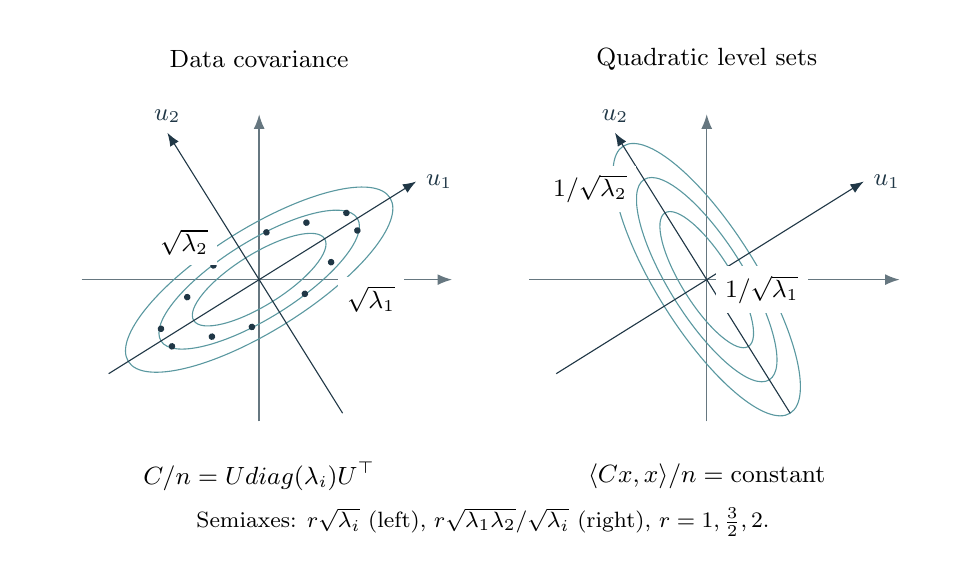
\begin{tikzpicture}[x=.98cm]
\pgfmathsetmacro{\lambdaone}{1}
\pgfmathsetmacro{\lambdatwo}{.325*.325}
\pgfmathsetmacro{\sigmaone}{sqrt(\lambdaone)}
\pgfmathsetmacro{\sigmatwo}{sqrt(\lambdatwo)}
\pgfmathsetmacro{\levelscale}{sqrt(\lambdaone*\lambdatwo)}
\path[use as bounding box] (-3,-3.25) rectangle (8.8,3.2);\begin{scope}[shift={(0.0,0)}]
\draw[axis] (-2.3,0)--(2.5,0);\draw[axis] (0,-1.8)--(0,2.1);\begin{scope}[rotate=32]
\foreach \r in {1,1.5,2} {
  \draw[accent!70] (0,0) ellipse ({\r*\sigmaone} and {\r*\sigmatwo});
}
\draw[->,ink] (-2.3,0)--(2.4,0) node[right] {$u_1$};\draw[->,ink] (0,-2.0)--(0,2.2) node[above] {$u_2$};
% Reflection symmetry gives zero mean and zero cross covariance.
% Since .4^2+.9^2+1.4^2=2.93, the empirical eigenvalues
% of these twelve points are exactly 1 and .325^2.
\foreach \a/\b in {.4/1.4,.9/.9,1.4/.4} {
  \foreach \sx in {-1,1} {
    \foreach \sy in {-1,1} {
      \fill[ink] ({\sx*\sigmaone*\a*sqrt(3/2.93)},{\sy*\sigmatwo*\b*sqrt(3/2.93)}) circle (1.2pt);
    }
  }
}
\node[below,fill=white] at (1.25,-.72) {$\sqrt{\lambda_1}$};\node[left,fill=white] at (-.2,.68) {$\sqrt{\lambda_2}$};\end{scope}\node at (0,2.8) {Data covariance};\node at (0,-2.5) {$C/n=U\operatorname{diag}(\lambda_i)U^\top$};
\end{scope}
\begin{scope}[shift={(5.8,0)}]
\draw[axis] (-2.3,0)--(2.5,0);\draw[axis] (0,-1.8)--(0,2.1);\begin{scope}[rotate=32]
\foreach \r in {1,1.5,2} {
  \draw[accent!70] (0,0) ellipse ({\r*\levelscale/\sigmaone} and {\r*\levelscale/\sigmatwo});
}
\draw[->,ink] (-2.3,0)--(2.4,0) node[right] {$u_1$};\draw[->,ink] (0,-2.0)--(0,2.2) node[above] {$u_2$};\node[below,fill=white] at (.7,-.22) {$1/\sqrt{\lambda_1}$};\node[left,fill=white] at (-.15,1.45) {$1/\sqrt{\lambda_2}$};\end{scope}\node at (0,2.8) {Quadratic level sets};\node at (0,-2.5) {$\langle Cx,x\rangle/n=\mathrm{constant}$};
\end{scope}
\node[align=center,font=\footnotesize] at (2.9,-3.08)
  {Semiaxes: $r\sqrt{\lambda_i}$ (left), $r\sqrt{\lambda_1\lambda_2}/\sqrt{\lambda_i}$ (right), $r=1,\frac32,2$.};
\end{tikzpicture}
\end{document}
